% Appendices here
% \newgeometry{top=0.5cm,bottom=0.5cm}
\section*{Model A Learning Curves - Greyscale Comparison}

\subsection*{Greyscale Applied To Gender \& Age Branches}
\begin{figure}[h!]
    \centering
    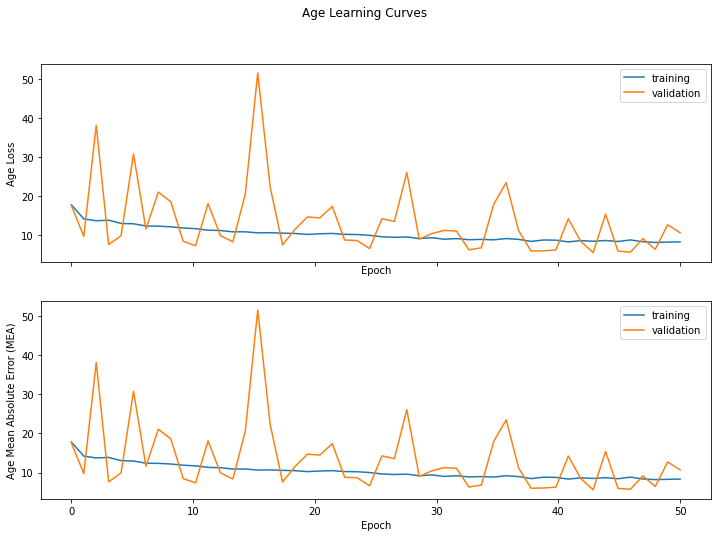
\includegraphics[height=0.42\textheight]{ModelA_AgeLearning_FCNDropout_BothGreyScale_NoRegularisation.png}
\end{figure}
\begin{figure}[h!]
    \centering
    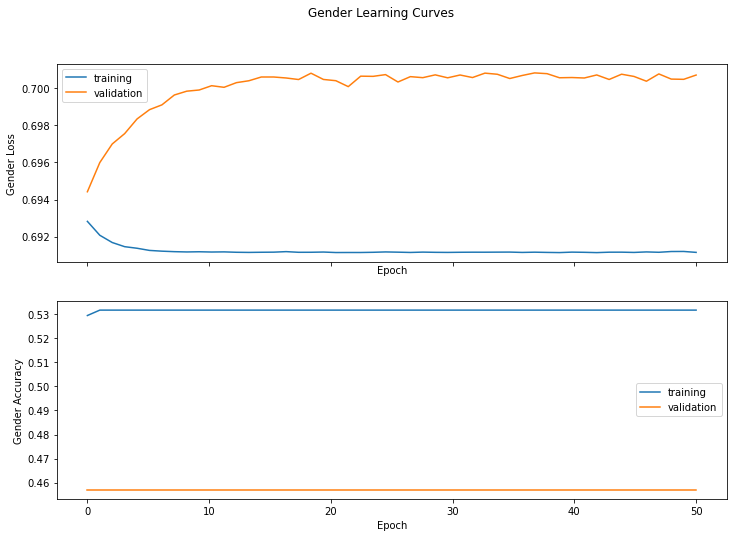
\includegraphics[height=0.42\textheight]{ModelA_GenderLearning_FCNDropout_BothGreyScale_NoRegularisation.png}
\end{figure}
\newpage

\subsection*{Greyscale Applied To Neither Branch}
\begin{figure}[h!]
    \centering
    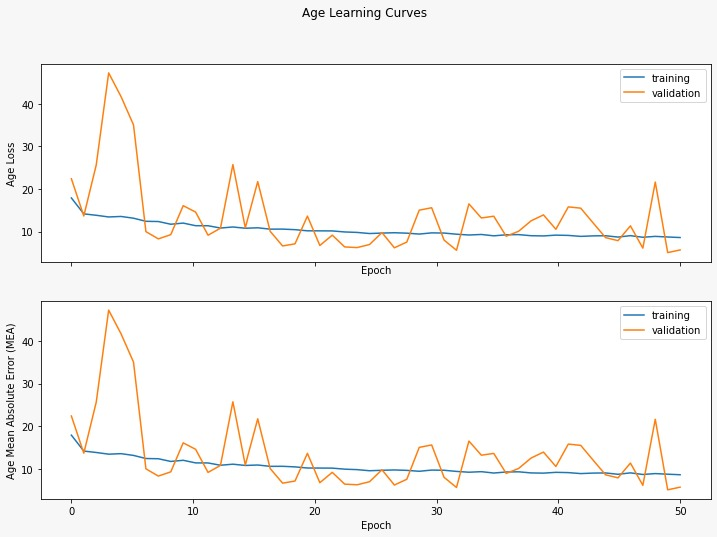
\includegraphics[height=0.42\textheight]{ModelA_AgeLearning_FCNDropout_NoGreyScale_NoRegularisation.jpeg}
\end{figure}
\begin{figure}[h!]
    \centering
    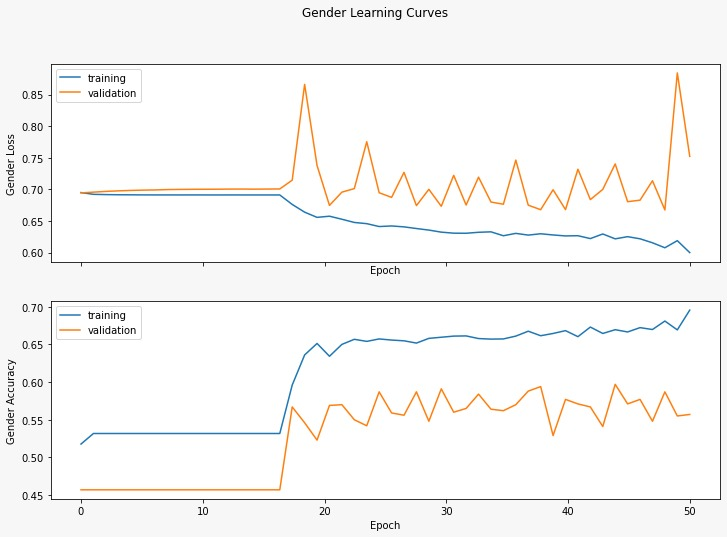
\includegraphics[height=0.42\textheight]{ModelA_GenderLearning_FCNDropout_NoGreyScale_NoRegularisation.jpeg}
\end{figure}
\newpage

\subsection*{Greyscale Applied To Gender Branch Only}
\begin{figure}[h!]
    \centering
    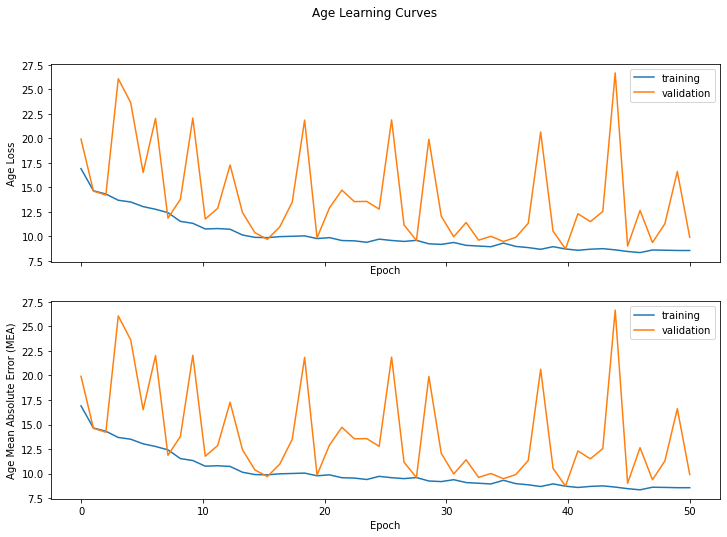
\includegraphics[height=0.42\textheight]{ModelA_AgeLearning_FCNDropout_GenderGreyScale_NoRegularisation.png}
\end{figure}
\begin{figure}[h!]
    \centering
    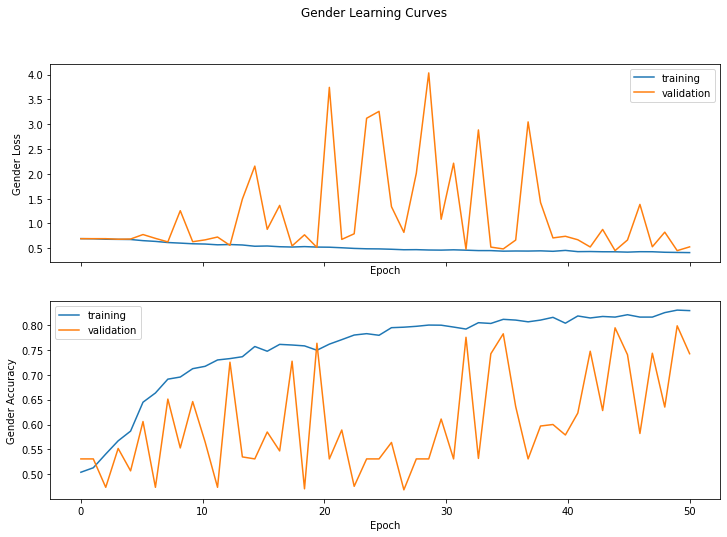
\includegraphics[height=0.42\textheight]{ModelA_GenderLearning_FCNDropout_GenderGreyScale_NoRegularisation.png}
\end{figure}
\newpage

\section*{Original Model A Graphs}
\subsection*{No Greyscale}
\begin{figure}[h!]
    \centering
    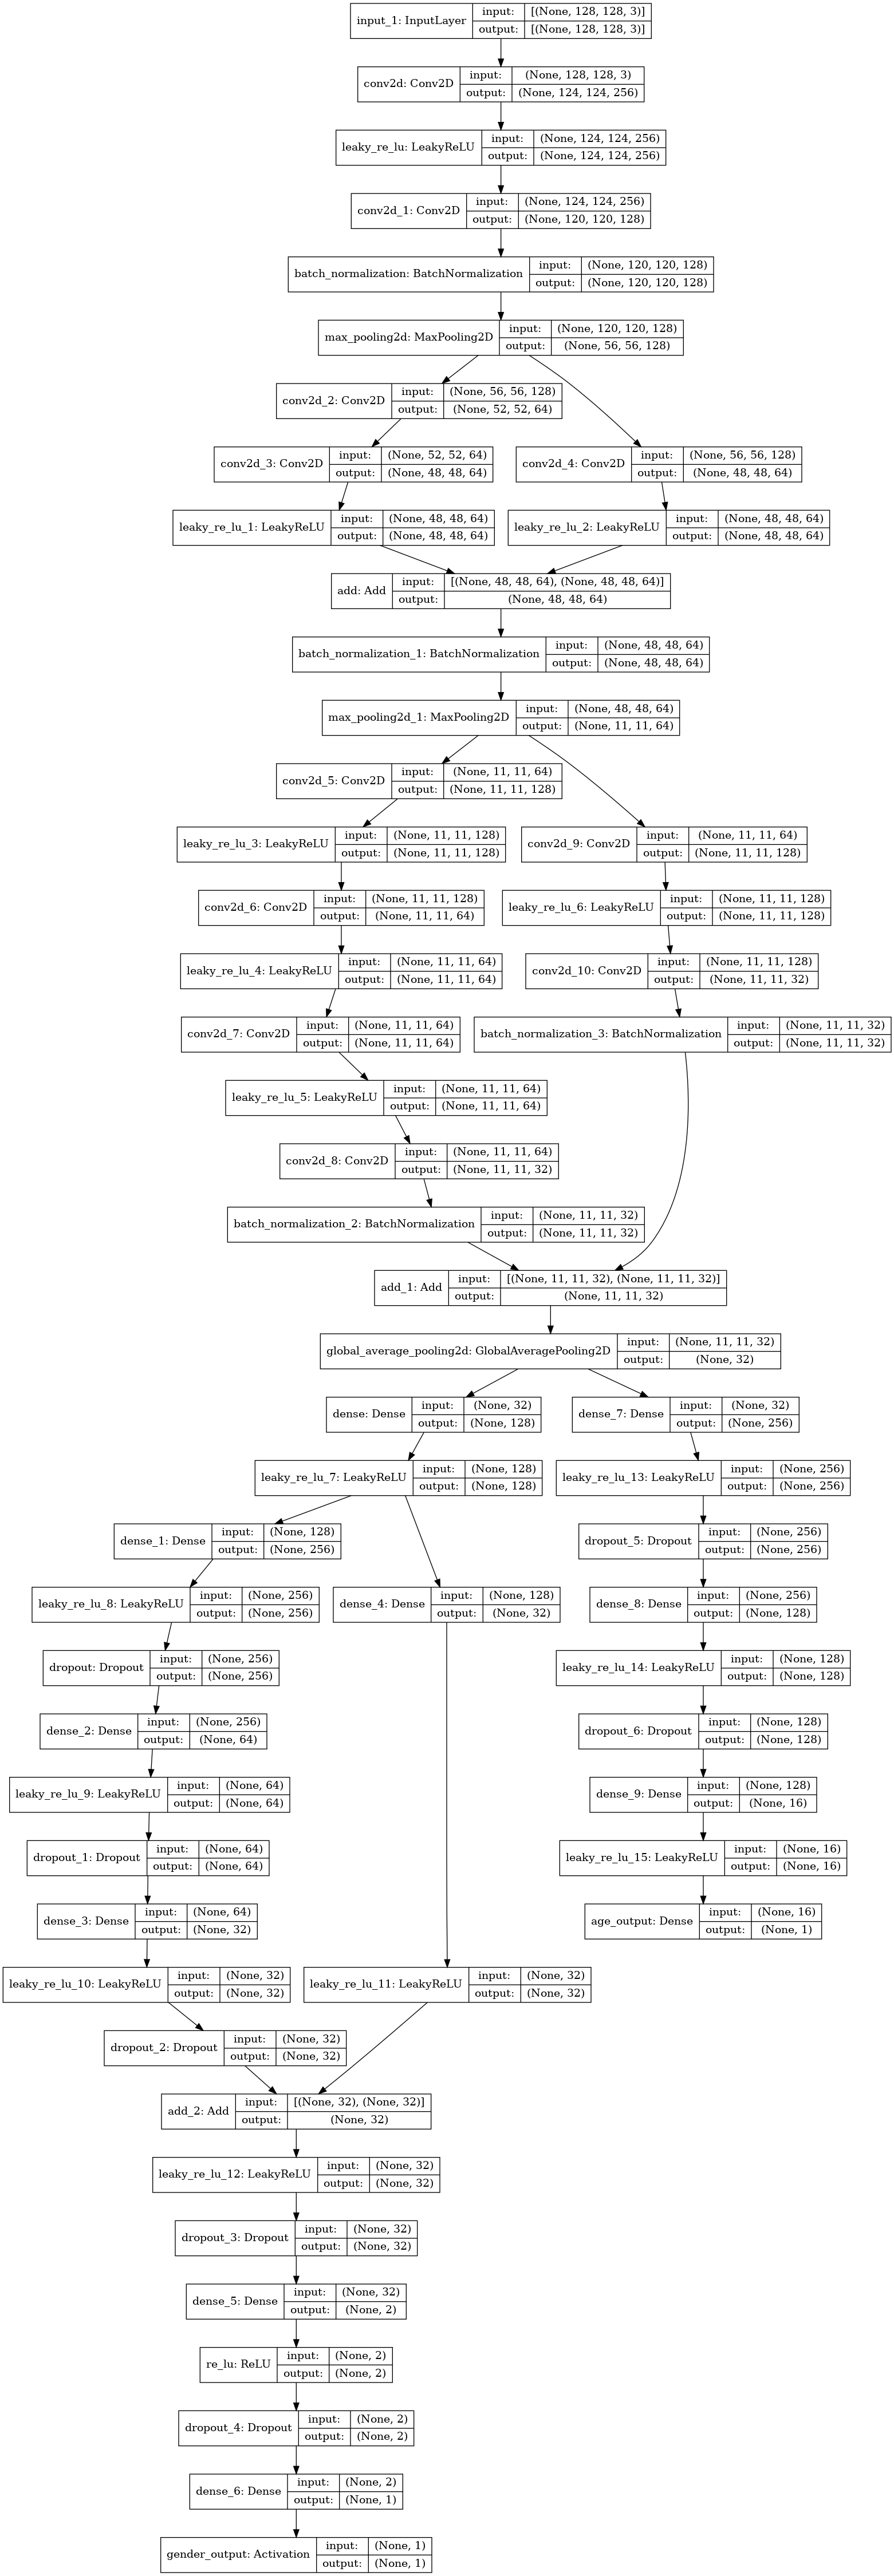
\includegraphics[height=0.9\textheight]{ModelAGraph_sample.png}
\end{figure}
\newpage

\subsection*{Greyscale Applied To Gender Branch Only}
\begin{figure}[h!]
    \centering
    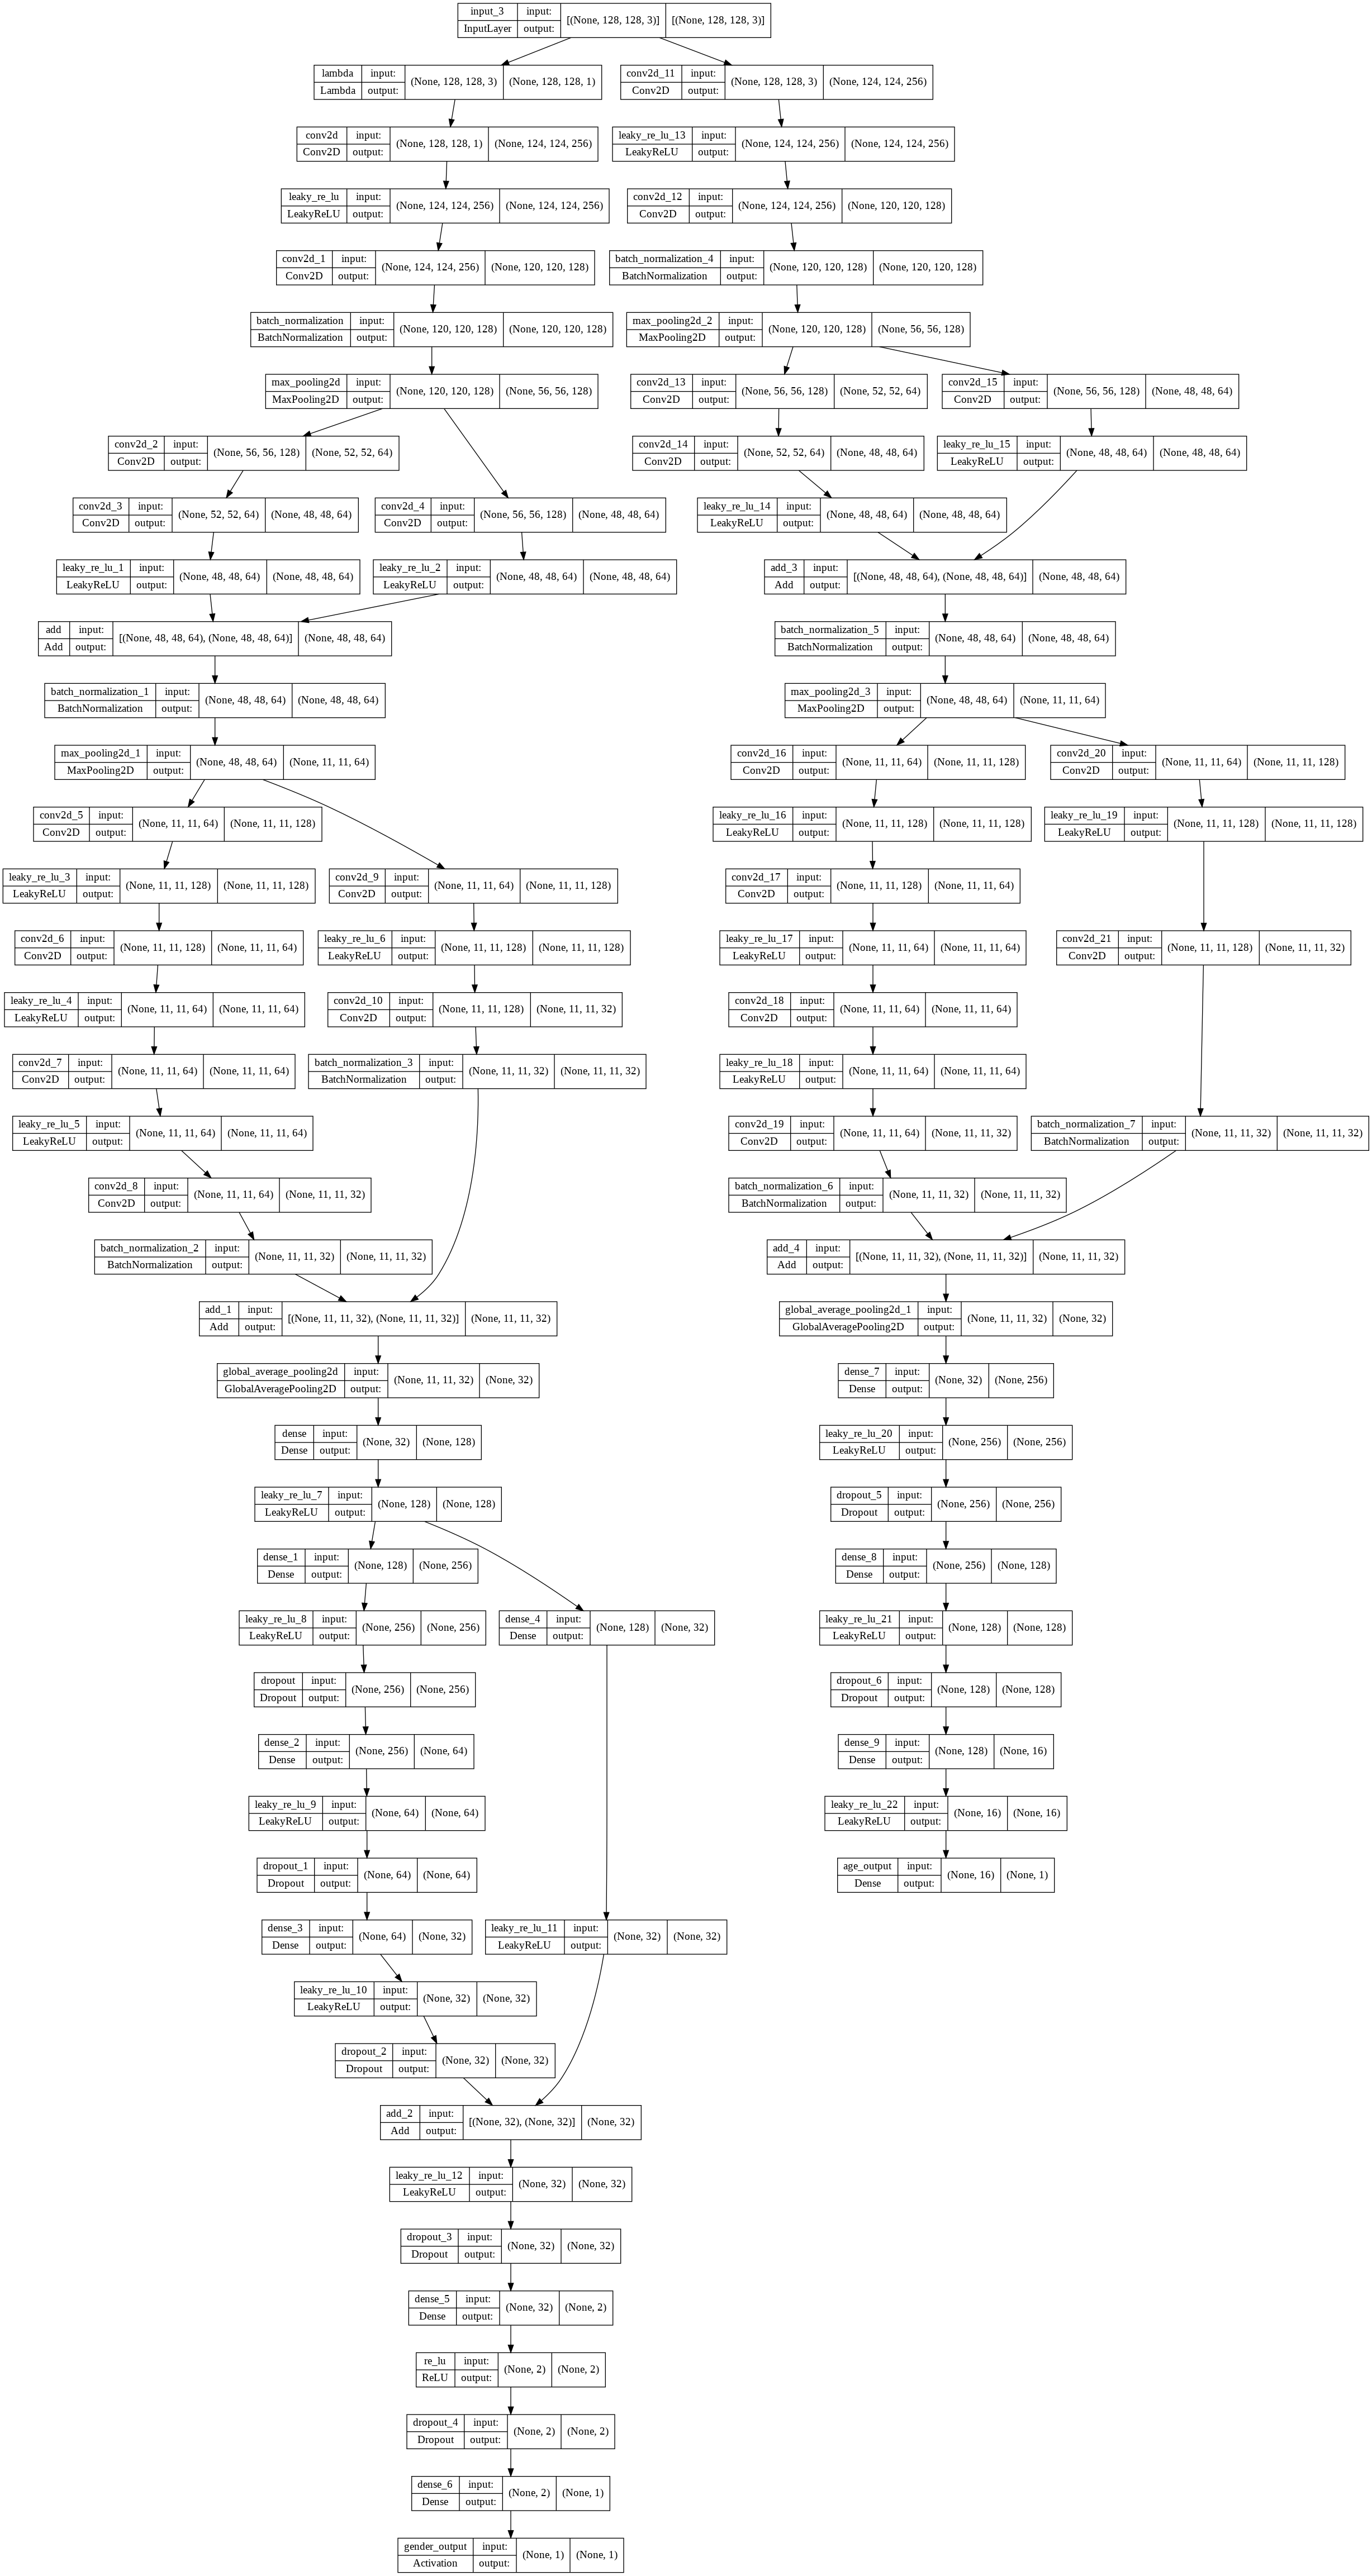
\includegraphics[height=0.9\textheight]{ModelAGraph_sample_GreyscaleGenderBranch.png}
\end{figure}
\newpage

\subsection*{Greyscale Applied To Both Branches}
\begin{figure}[h!]
    \centering
    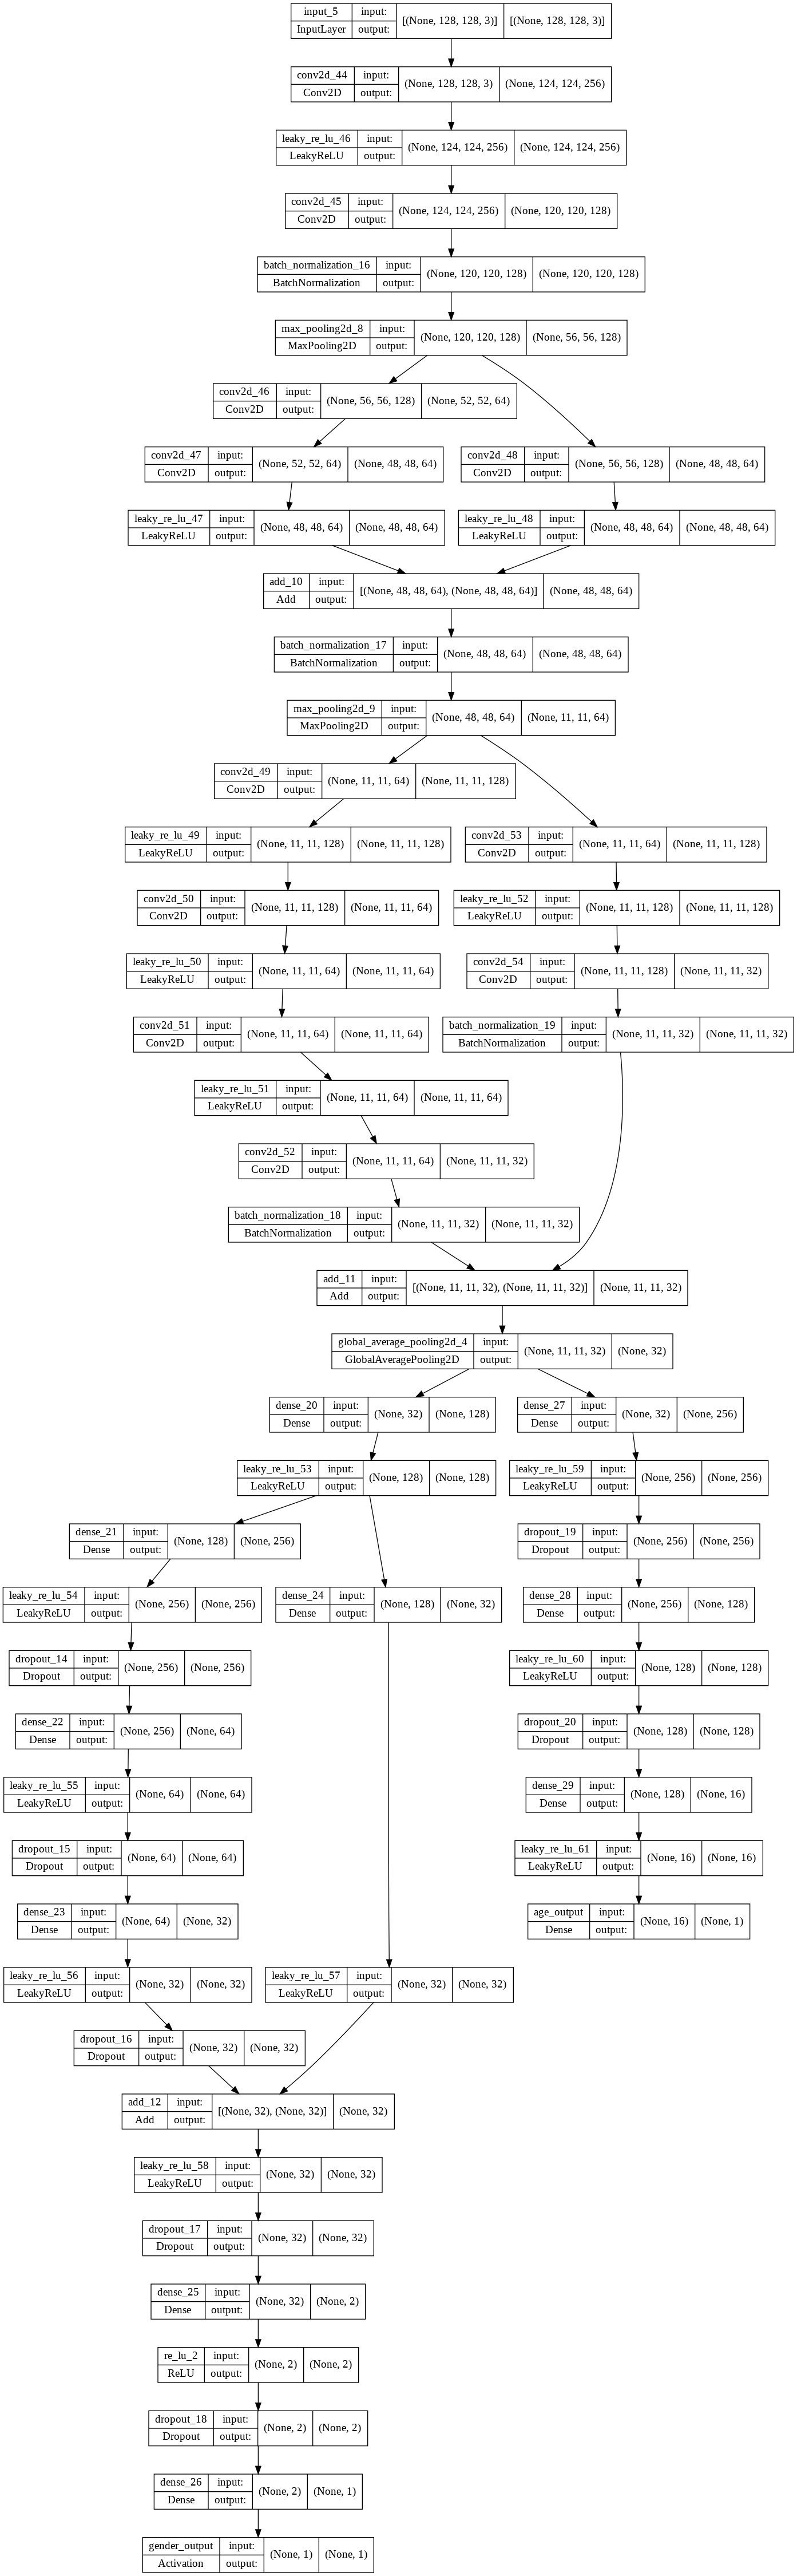
\includegraphics[height=0.9\textheight]{ModelAGraph_sample_GreyscaleBothBranches.png}
\end{figure}
\newpage
